\documentclass[preprint,12pt]{elsarticle}

\usepackage{amsmath}
\usepackage{amssymb}
\usepackage{booktabs}
\usepackage{array}
\usepackage{tabularx}
\usepackage{siunitx}
\usepackage{microtype}
\usepackage{placeins}
\usepackage{graphicx}
\setlength{\emergencystretch}{2em}
\newcolumntype{Y}{>{\centering\arraybackslash}X}

\journal{Digital Signal Processing}

\begin{document}

\begin{frontmatter}

\title{Background-Conditioned CFAR for Reliable Radar Target Detection in Nonstationary Sea Clutter}

\author[aff1]{Zixuan Liu}
\author[aff2,aff3]{Wei Xiong\corref{cor1}}
\ead{xw@mail.hbut.edu.cn}

\cortext[cor1]{Corresponding author}

\affiliation[aff1]{organization={Detroit Green Technology Institute, Hubei University of Technology},
            addressline={},
            city={Wuhan},
            postcode={430068},
            state={},
            country={China}}
\affiliation[aff2]{organization={School of Electrical and Electronic Engineering, Hubei University of Technology},
            addressline={},
            city={Wuhan},
            postcode={430068},
            state={},
            country={China}}
\affiliation[aff3]{organization={Department of Computer Science and Engineering, University of South Carolina},
            addressline={},
            city={Columbia},
            postcode={SC 29201},
            state={},
            country={USA}}

\begin{abstract}
False-alarm control is central to radar target detection under nonstationary sea
clutter. A detector can match the nominal rate after many trials are pooled
while still producing acquisition-specific bursts of false alarms. We introduce
BC-DRCFAR, a background-conditioned CFAR detector that uses
same-time reference clutter to refine detection scores and set thresholds.
BC-DRCFAR represents the background with distributional, temporal, tail-shape,
and reference-series features and couples them to a scale-equivariant detection
branch. Thresholds are calibrated directly to the declared false-alarm operating
point.
On the full-budget synthetic benchmark, BC-DRCFAR reduces the factor-2
false-alarm violation rate from 83.3\% for GO-CFAR to 18.8\%, lowers the mean
absolute log10 false-alarm error from 1.070 to 0.174, and raises the detection
probability at 0 dB from 0.740 to 0.835. On retrospective IPIX sea-clutter
acquisitions, the feature-head calibration keeps the macro false-alarm
probability close to the nominal level and improves acquisition-level
calibration over scalar and GO baselines. Observed clutter background can
thereby move CFAR beyond a local thresholding rule and make it a reliable
calibration mechanism for nonstationary sea clutter.
\end{abstract}

\begin{highlights}
\item Background-conditioned CFAR calibration targets acquisition-level reliability.
\item BC-DRCFAR reduces factor-2 false-alarm violations on synthetic sea clutter.
\item Retrospective IPIX results improve acquisition-level false-alarm calibration.
\item Robustness audits characterize temporal and domain reliability.
\end{highlights}

\begin{keyword}
sea clutter \sep radar target detection \sep constant false alarm rate \sep probability of false alarm \sep background-conditioned calibration \sep IPIX radar data
\end{keyword}

\end{frontmatter}

\section{Introduction}
\label{sec:introduction}

Reliable maritime radar target detection requires weak targets to be detected
while false alarms stay at the declared operating point. Sea clutter makes this a
calibration problem because the background return changes with sea state,
grazing geometry, polarization, and acquisition conditions
\cite{ward2013seaclutter,watts2008seaclutter,greco2006polarimetric,greco2010nonstationarity}.
A detector can show
an acceptable average false-alarm probability after pooling many trials and
still produce bursts of false alarms in individual acquisitions. For practical
surveillance, this acquisition-level behaviour is the case operators encounter.

The declared false-alarm probability is more than a tuning parameter. It is the
quantity that connects a detector to downstream tracking, display load, and
operator response. When the empirical false-alarm rate drifts between
acquisitions, the detector no longer provides the operating point promised by
its threshold. This effect is especially important for small maritime targets,
where raising the threshold to suppress clutter spikes can remove precisely the
low signal-to-clutter returns that the detector is meant to preserve. Reliable
sea-clutter detection therefore requires two capabilities at the same time:
ranking target evidence and keeping the declared false-alarm rate meaningful in
the background currently being observed.

Constant false-alarm rate (CFAR) detection remains the standard tool for this
problem. Classical cell-averaging and greatest-of CFAR detectors estimate a
local clutter level and set thresholds to meet a declared false-alarm
probability \cite{rohling1983cfar,hansen1980go,kelly1986adaptive}. Their simplicity and clear
operating-point interpretation make them strong baselines. In nonstationary sea
clutter, heavy-tailed and mismatched reference cells directly disrupt threshold
calibration. This turns false-alarm control from a local power-estimation
problem into a background-conditioned calibration problem.

The key technical difficulty is that the reference window has two roles. It
provides the samples from which the clutter level is estimated, and it also
reveals the condition under which the threshold will be used. Classical CFAR
mostly compresses this window into a scalar summary, such as an average, an
order statistic, or a greatest-of estimate. That summary is effective when the
background is close to the assumed model. In measured sea clutter, the same
window can also contain information about tail weight, temporal persistence,
range-bin mismatch, and polarization-dependent clutter structure. Treating that
information as a calibration signal is the central move in this paper.

Recent work has improved radar detection in heterogeneous and non-Gaussian sea
clutter through adaptive CFAR variants, statistical clutter modelling,
feature-based detection, and learning-based detectors
\cite{xue2022adaptive,rihan2024cfar,mungara2024heterogeneous,conte2002recursive,sangston2012heavytailed}.
These methods
have advanced robustness in important regimes. A gap remains at the calibration
stage: the same background structure used for detection should also inform the
declared false-alarm operating point. BC-DRCFAR develops this idea by
conditioning calibration on the observed clutter structure that drives
acquisition-specific false alarms.

We propose BC-DRCFAR as a background-conditioned CFAR framework for reliable
radar target detection in nonstationary sea clutter. The method uses same-time
reference clutter to condition both score refinement and threshold adjustment.
It represents the background using distributional, temporal, tail-shape, and
reference-series features, then couples these features to a scale-equivariant
detection branch. The resulting detector keeps the CFAR operating-point
interpretation while adding a learned calibration mechanism driven by the
clutter background observed at detection time.

The main contributions are as follows.
\begin{itemize}
\item We formulate sea-clutter false-alarm control as an acquisition-level
calibration problem, exposing failures that can be hidden by pooled
$P_{\mathrm{fa}}$ summaries.
\item We propose a background-conditioned CFAR architecture that jointly refines
detection scores and calibrates thresholds from same-time reference clutter.
\item We combine distributional, temporal, tail-shape, and reference-series
background descriptors with a scale-equivariant detection branch, giving the
model direct access to the clutter structure that governs false-alarm
instability.
\item We validate BC-DRCFAR on a full-budget synthetic benchmark and
retrospective McMaster IPIX sea-clutter acquisitions, showing improved
false-alarm calibration over GO-CFAR and scalar calibration baselines.
\end{itemize}

\section{Related work}
\label{sec:related-work}

\subsection{CFAR detection in heterogeneous sea clutter}

CFAR detection is the standard radar framework for converting a desired
false-alarm probability into an adaptive threshold. Classical CA-CFAR,
GO-CFAR, SO-CFAR, and OS-CFAR variants differ mainly in how the reference
window is summarized and how interference or clutter edges are handled
\cite{hansen1980go,rohling1983cfar,barkat1989multiple}. This design gives CFAR
detectors a clear operational interpretation, which is why they remain strong
baselines in sea-clutter studies.

Maritime clutter often departs from the homogeneous background assumptions that
make simple reference-window estimates reliable. High-resolution sea clutter can
be heavy-tailed, non-Gaussian, and heterogeneous across adjacent range cells and
acquisitions. Much of the CFAR literature addresses this by adopting more
suitable clutter models or more robust reference-cell processing. Examples
include heavy-tailed texture models, K-distributed clutter modelling,
heterogeneous-clutter CFAR design, and
environment-adaptive thresholding
\cite{sekine1983weibull,watts1987spatial,xue2022adaptive,zhao2019dbscan,mungara2024heterogeneous,rihan2024cfar,xiao2024alternate,aldabaa2025multiple,hop2025twostage}.
These methods establish the value of adapting CFAR to clutter statistics.
BC-DRCFAR extends this line of work by treating the background as a conditioning
variable for calibration, so that threshold adjustment is driven by the observed
clutter structure at detection time.

The difference becomes clear at the acquisition level. Classical CFAR analysis
usually emphasizes the threshold factor implied by a clutter model and a target
false-alarm probability. In measured sea clutter, the same nominal setting can
produce different false-alarm behaviour across acquisitions because the
reference cells carry different tail, correlation, and mismatch structure.
BC-DRCFAR uses this acquisition-specific structure directly. It preserves the
CFAR idea of declaring an operating point while allowing the calibration rule to
respond to the observed reference background.

This acquisition-level view also changes how methods should be compared. A
detector can match the nominal $P_{\mathrm{fa}}$ after all clutter cells are
pooled and still be unreliable in the individual acquisition that generated the
alarms. For that reason, the relevant comparison must include the threshold
formula, the pooled false-alarm rate, and the stability of the declared
operating point across acquisitions. BC-DRCFAR is built for this comparison: the
input is the same reference background used by CFAR, and the output remains a
thresholded decision at a declared $P_{\mathrm{fa}}$.

\subsection{Feature-based and statistical sea-clutter detection}

Another line of work improves maritime target detection by describing sea
clutter with richer statistics before applying a detector. Filtering-then-CFAR
methods suppress clutter in the spatio-temporal or frequency-wavenumber domain
and then design a detector for the filtered background
\cite{wen2022spatiotemporal,wen2024gev}. Other approaches model nonlinear
feature dependence or exploit multi-channel observations. Copula-based CFAR
methods, for example, use feature dependence to derive detection statistics and
false-alarm probabilities for multi-feature or dual-polarization detection
\cite{li2025copula,jiang2025twodcfar,fan2024fullpolarization}.

These studies show that background structure carries information beyond a single
amplitude estimate. BC-DRCFAR uses that structure for calibration as well as
detection. Its distributional, temporal, tail-shape, and reference-series
descriptors condition both score refinement and threshold selection.

This also separates the proposed detector from feature-only decision rules.
Feature-based detectors often improve the separation between target and clutter
returns, but the link between a multidimensional feature space and a declared
$P_{\mathrm{fa}}$ can become indirect. BC-DRCFAR keeps that link explicit by
using background descriptors to set the threshold itself. The features are not
only evidence for the target class; they are evidence about the clutter state
under which the threshold must operate.

The distinction is important for sea clutter because the same feature can have
different decision meaning under different backgrounds. A high-amplitude return
inside a calm, weak-tailed reference window is different from a high-amplitude
return inside a spiky, correlated, or polarization-shifted background. A
feature-only detector tends to ask whether the CUT is target-like. A
background-conditioned CFAR detector also asks what threshold is justified by
the clutter condition around that CUT. This makes feature extraction part of the
false-alarm calibration mechanism and ties the features directly to the
operating point \cite{luo2022lowobservable,guan2024nonlinear,yang2017polarization}.

\subsection{Learning-based radar target detection}

Learning-based radar detectors have been introduced to capture target--clutter
differences that are difficult to express with fixed statistical models.
Recent methods combine reconstruction, multi-domain features, neural networks,
or geometric representations to improve detection under complex sea clutter
\cite{liang2022unsupervised,wang2023sala,wang2024triplechannel,wang2025twostage,chen2025multidomain,chen2026mspmig,bai2026complexvae}.
These approaches can absorb
heterogeneous inputs and learn discriminative representations from measured
data.

For radar deployment, the decision threshold must correspond to a reliable
false-alarm operating point. BC-DRCFAR places declared $P_{\mathrm{fa}}$
calibration at the center of the method. It keeps the CFAR operating-point
language and uses a learned background-conditioned mechanism to improve
acquisition-level false-alarm reliability in nonstationary sea clutter.

The contribution is complementary to learning-based representation methods. A
detector may learn a strong score and still require a calibration rule that
remains meaningful from acquisition to acquisition. BC-DRCFAR makes this rule
part of the model. The score branch orders target evidence, and the threshold
branch maps the declared operating point to the local clutter condition. This
design gives the learned detector a CFAR-style operating interface instead of a
free classification threshold.

This paper therefore connects two lines of radar signal processing that are
often treated separately. Classical CFAR supplies a disciplined operating
interface through $P_{\mathrm{fa}}$, while modern feature learning supplies a
way to represent clutter structure beyond a scalar reference estimate.
BC-DRCFAR keeps the operating interface and uses the learned representation only
where it is most useful: calibrating the threshold for the observed background.

\section{Method}
\label{sec:method}

\subsection{Detection problem and CFAR operating point}
\label{subsec:problem}

For each cell under test (CUT), the detector receives a complex radar sample and
a set of same-time reference cells from the same acquisition. Let $x$ denote the
CUT and let $R=\{r_i\}_{i=1}^{K}$ denote the reference set. The task is target
detection at a declared false-alarm operating point $\alpha$.

We write the detector as a score function and a threshold function. The score
$s(x,R)$ measures target evidence in the CUT under its local clutter context.
The threshold $\tau(R;\alpha)$ maps the same context and the declared
false-alarm probability to a decision level. A detection is declared by
\begin{equation}
  d(x,R;\alpha) = \mathbb{1}\{s(x,R) > \tau(R;\alpha)\}.
  \label{eq:decision-rule}
\end{equation}
This form preserves the CFAR operating-point language while allowing the
threshold to depend on the observed background structure.

The formulation separates two quantities that are often coupled in practice:
target evidence and false-alarm calibration. The score $s(x,R)$ ranks how
target-like the CUT appears under its local context. The threshold
$\tau(R;\alpha)$ expresses the decision level required by the declared
operating point in that same context. This separation lets BC-DRCFAR improve the
ordering of candidate cells without losing the CFAR interpretation of the final
binary decision.

\subsection{Overview of BC-DRCFAR}
\label{subsec:overview}

BC-DRCFAR separates background description, CUT scoring, and threshold
calibration. The background branch extracts descriptors from the same-time
reference clutter. The CUT branch computes target evidence for the test cell and
conditions that evidence on the background representation. The threshold branch
then maps the same background representation and target $\alpha$ to the decision
level used in Eq.~\eqref{eq:decision-rule}.

After training, the inference path is fixed. Given $(x,R,\alpha)$, the detector
forms a background representation from $R$, refines the CUT score under that
background, evaluates the calibrated threshold, and compares the two quantities.
The background enters the detector as an explicit calibration variable.

The architecture is built around the same information available to a CFAR
detector at test time. Calibration factors and feature-head parameters are fixed
before retrospective scoring. Acquisition-specific behaviour is then carried by
the measured reference background. This fixed inference path makes the IPIX
evaluation a direct test of calibration transfer.

The resulting pipeline has a simple operational interpretation. The reference
cells are first converted into a background representation. The CUT is then
scored relative to that representation. Finally, the declared operating point
$\alpha$ is converted into a threshold that is specific to the same background.
The method therefore keeps the CFAR decision form and upgrades the calibration
step from a scalar threshold correction to a background-conditioned threshold
function.

Figure~\ref{fig:method-overview} summarizes this data flow and fixes the role of
each module before the module-level description. The background encoder, score
branch, threshold branch, and final score-threshold comparison together form a
single CFAR-style decision rule rather than a detached scoring network.

\begin{figure}[!htbp]
\centering
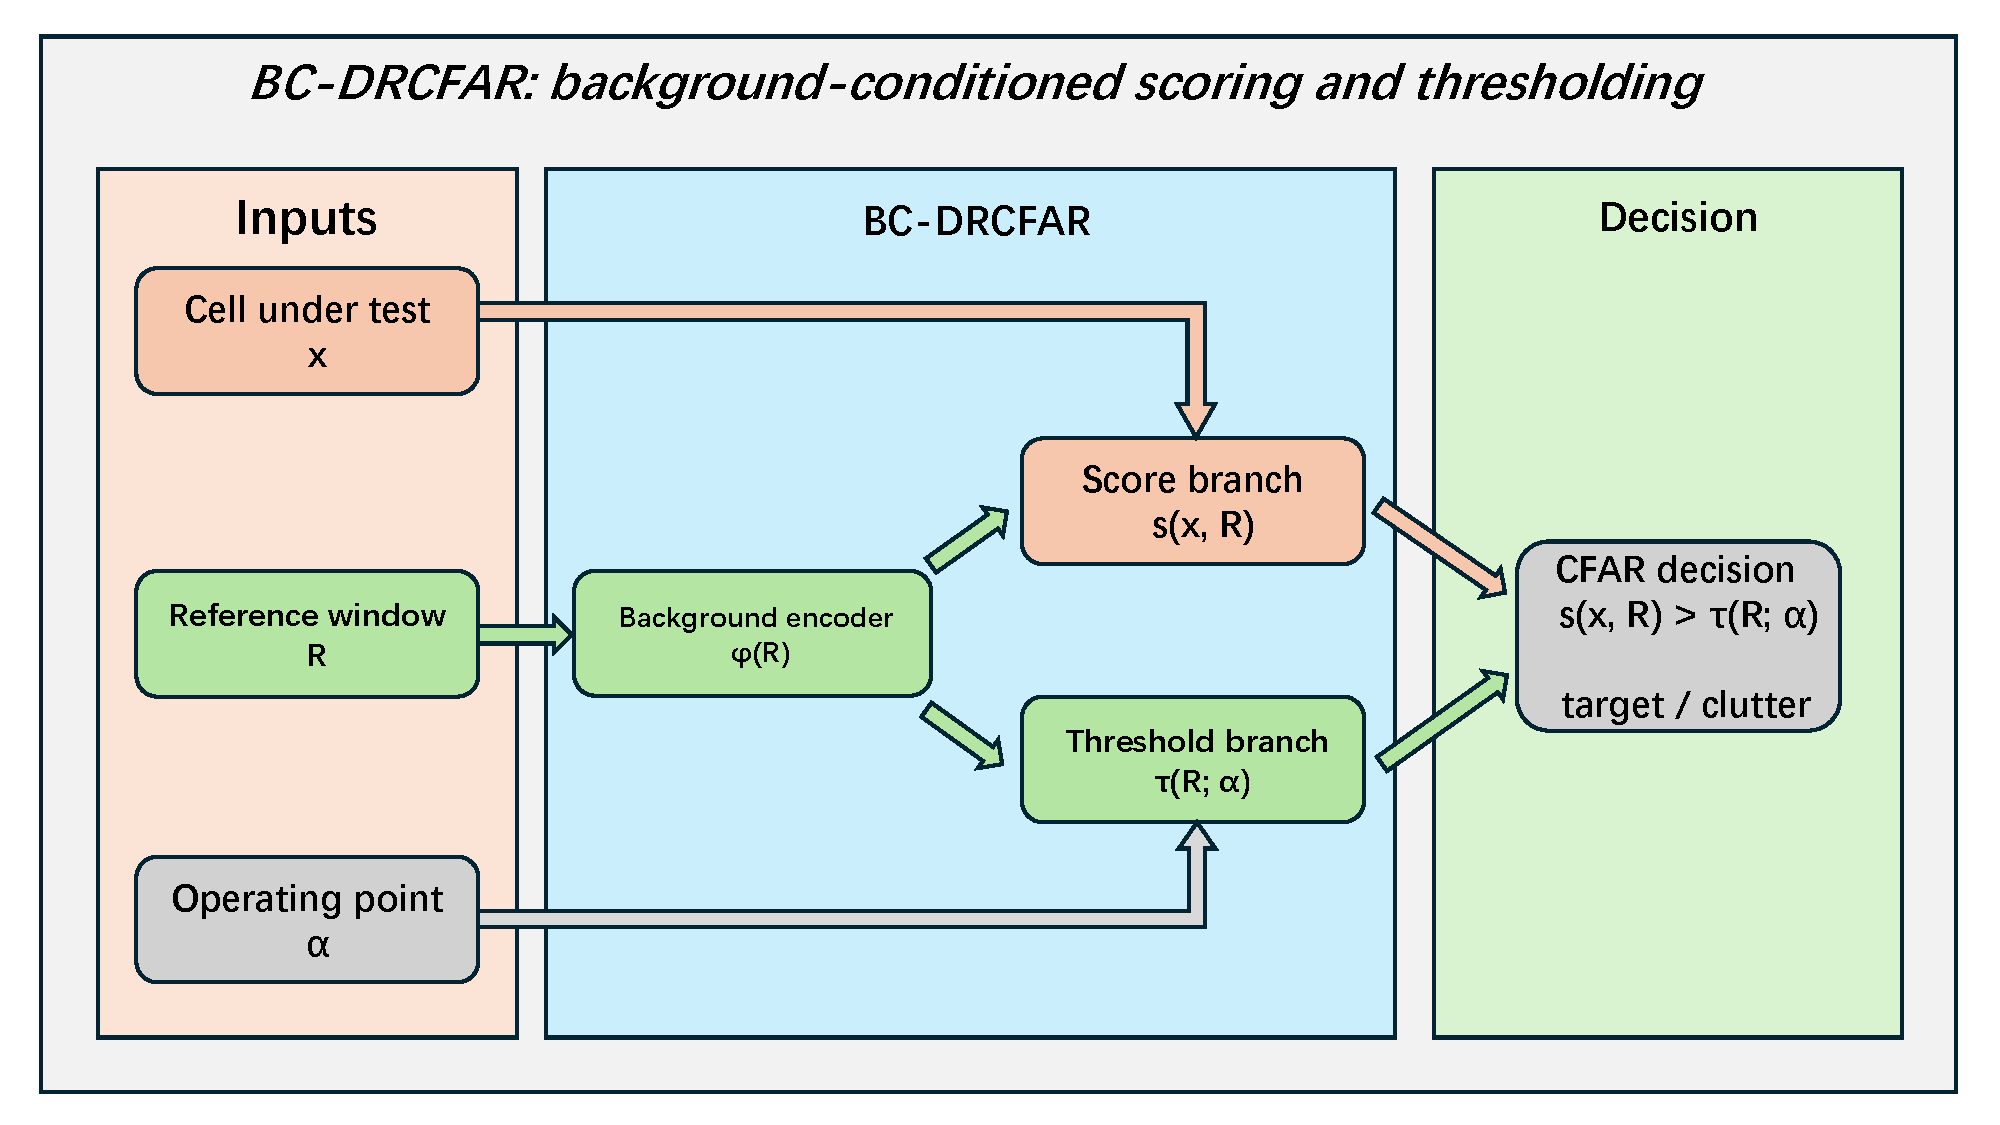
\includegraphics[width=\textwidth]{fig1_method_overview.pdf}
\caption{Overview of BC-DRCFAR. Same-time reference clutter is represented by
distributional, temporal, tail-shape, and reference-series descriptors. The
background representation conditions both the CUT score and the threshold used
for the declared false-alarm operating point.}
\label{fig:method-overview}
\end{figure}
\FloatBarrier

\subsection{Background representation}
\label{subsec:background-features}

The background branch summarizes the same-time reference clutter with four
descriptor groups. Distributional descriptors record the amplitude level and
spread of the reference cells. Temporal descriptors record dependence across the
available slow-time samples. Tail-shape descriptors record heavy-tailed and
spiky behaviour in high-resolution sea clutter. Reference-series descriptors
retain information from the ordered reference sequence, so the background is not
collapsed to a single power estimate.

Each descriptor group has a distinct calibration role. Distributional
descriptors anchor the scale of the local clutter. Temporal descriptors capture
slow-time persistence, which changes how isolated high returns should be
interpreted. Tail-shape descriptors summarize the tendency of sea clutter to
produce spikes that resemble target returns. Reference-series descriptors keep
the ordering and local contrast information that is lost when the reference
window is reduced to one average or order statistic.

Let $\phi(R)$ denote the concatenated background descriptor vector. BC-DRCFAR
uses $\phi(R)$ as the conditioning variable for both score refinement and
threshold calibration:
\begin{equation}
  z_R = g_{\theta}(\phi(R)),
\end{equation}
where $g_{\theta}$ is the background encoder and $z_R$ is the fused clutter
representation. This vector carries the background factors used later for
score refinement and threshold calibration.

The same $z_R$ is shared by the score and threshold branches. Sharing the
background representation makes the two branches respond to the same observed
clutter state. When the background is heavy-tailed, shifted, or temporally
correlated, both the target-evidence score and the decision threshold are
conditioned on that state instead of being calibrated from a pooled average.

The four descriptor groups are intentionally redundant at the level of raw
information but distinct at the level of calibration role. Distributional
features supply the local scale and spread that classical CFAR estimates with a
single statistic. Temporal features describe slow-time dependence, which affects
the chance that a high return is part of a persistent clutter process.
Tail-shape features capture spikiness and asymmetric high-end behaviour, the
main source of false alarms in heavy-tailed clutter. Reference-series features
preserve ordered local structure across nearby non-target cells, giving the
threshold branch access to mismatch patterns that are lost in scalar averaging.

\subsection{Scale-equivariant score refinement}
\label{subsec:score-refinement}

The CUT branch computes a base target-evidence score from the test cell and its
reference context. Radar amplitudes can vary substantially across acquisitions,
so the score path is designed to preserve the decision structure under common
amplitude rescaling. In practice, the CUT branch operates on normalized CUT and
reference statistics and is coupled to $z_R$ before the final score is produced:
\begin{equation}
  s(x,R) = f_{\theta}(x,R,z_R).
\end{equation}
This branch provides the target-evidence ordering used by the final CFAR
decision.

Scale equivariance is used to keep the score meaningful across acquisitions
with different amplitude ranges. If both the CUT and its reference background
are scaled by a common factor, the normalized statistics preserve the relative
target evidence seen by the branch. The final threshold can then handle the
declared false-alarm operating point without forcing the score branch to learn a
new absolute scale for every acquisition \cite{kraut1999scale}.

\subsection{Background-conditioned threshold calibration}
\label{subsec:threshold-calibration}

The threshold branch is the calibration core of BC-DRCFAR. For a declared
false-alarm probability $\alpha$, the branch predicts a threshold from the
background representation:
\begin{equation}
  \tau(R;\alpha) = h_{\theta}(z_R,\alpha).
\end{equation}
The threshold function is anchored to monotone $P_{\mathrm{fa}}$ operating
points. Lower target false-alarm probabilities correspond to stricter
thresholds, and the learned correction adjusts the threshold according to the
observed clutter structure. The score path orders candidate CUTs, while the
threshold path maps the declared operating point to the acquisition-specific
decision level.

The calibration branch is anchored by analytic CFAR-style summaries before the
background-conditioned correction is applied. The anchor set includes summaries
based on CA power, trimmed power, Rayleigh median behaviour, Weibull log-moment
behaviour, upper order statistics, and robust high-quantile reference levels.
These anchors give the threshold branch a physically interpretable starting
point across common clutter regimes. The learned residual then adjusts the
threshold multiplicatively as a function of $z_R$ and $\alpha$, keeping the
correction tied to the declared false-alarm scale and separate from an
arbitrary classification score.

This design gives the method a direct link to CFAR practice. The user still
chooses an operating point $\alpha$, and the detector still returns a binary
decision by comparing a score with a threshold. The learned component changes
how the threshold is calibrated for the observed background. In this sense,
BC-DRCFAR keeps the operational interface of CFAR while replacing scalar
threshold adjustment with background-conditioned calibration.

\subsection{Staged training and inference}
\label{subsec:training-inference}

Training is staged to keep detection and calibration identifiable. Stage A
learns the score path on the development split. The score definition is then
frozen. Stage B trains residual CUT conditioning and the threshold-calibration
branch with the score path fixed. At test time, the frozen model receives
$(x,R,\alpha)$, computes $\phi(R)$ and $z_R$, evaluates $s(x,R)$ and
$\tau(R;\alpha)$, and returns the decision from Eq.~\eqref{eq:decision-rule}.

The staged procedure gives each training phase a clear role. Stage A learns a
stable ordering of CUT evidence. Stage B then learns how much the decision
level should move for the declared $P_{\mathrm{fa}}$ under the observed
background. Freezing the score before threshold calibration prevents the model
from hiding calibration changes inside the score scale. The final detector is
therefore a fixed decision rule at evaluation time.

Model selection follows the reliability objective used in the paper. Candidate
checkpoints are compared first by acquisition-level factor-2 violation rate and
log-scale false-alarm error, then by matched-operating-point detection
probability, parameter count, and latency. This ordering makes calibration
stability the primary selection criterion and treats detection probability as a
paired requirement at the same declared $P_{\mathrm{fa}}$. The parameter budget
is capped at 500,000 trainable parameters, so the reported gains are tied to the
calibration design and a compact model class.

\subsection{Reliability metrics}
\label{subsec:reliability-metrics}

The primary reliability endpoint is acquisition-level false-alarm calibration.
For each acquisition or series, the empirical false-alarm probability
$\widehat{P}_{\mathrm{fa}}$ is compared with the declared target $\alpha$. We
report the factor-2 violation event
\begin{equation}
  \widehat{P}_{\mathrm{fa}} < \frac{\alpha}{2}
  \quad \text{or} \quad
  \widehat{P}_{\mathrm{fa}} > 2\alpha.
\end{equation}
We also report the mean absolute log10 false-alarm error and detection
probability $P_{\mathrm{d}}$ at the specified signal-to-clutter ratio. These
metrics separate pooled calibration, acquisition-level calibration, and
detection probability.

The factor-2 event is used because it is directly interpretable at the
operating-point level. A detector with good pooled $P_{\mathrm{fa}}$ can still
violate the declared rate in many individual acquisitions. Mean absolute
log10-$P_{\mathrm{fa}}$ error measures the size of these deviations on the
natural scale for false-alarm probabilities. Reporting $P_{\mathrm{d}}$
alongside these calibration metrics keeps the detection trade-off visible.

\section{Experiments}
\label{sec:experiments}

\subsection{Experimental design}
\label{subsec:experimental-design}

The experiments follow the reliability problem addressed by BC-DRCFAR. We first
use a controlled nonstationary sea-clutter benchmark to measure
acquisition-level false-alarm calibration. We then move to public retrospective
IPIX acquisitions and keep the calibration artifacts frozen. Ablations and
reliability audits separate the effect of background conditioning from scalar
calibration and standard GO-CFAR thresholding.

All reported evaluations use locked data splits and fixed operating points. The
main target false-alarm probability is $P_{\mathrm{fa}}=0.01$. Two stricter
operating points, $P_{\mathrm{fa}}=0.003$ and $P_{\mathrm{fa}}=0.001$, are also
reported on the synthetic benchmark. The main comparison is made at the
acquisition level, where false-alarm bursts directly determine operational
reliability.

The evaluation protocol is deliberately tied to the operating point and to
acquisition-level reliability. For each method, the declared
$P_{\mathrm{fa}}$ is fixed before scoring. The observed false-alarm probability
is then measured both after pooling all cells and within each acquisition. This
layout exposes the practical calibration question: a radar detector must keep
the declared operating point in the series being processed as well as in the
pooled summary.

\subsection{Synthetic nonstationary sea-clutter benchmark}
\label{subsec:synthetic}

The synthetic benchmark contains seven clutter scenarios:
candidate-family, gamma-shape shift, inverse-gamma $G^0$, correlated,
contaminated, mixture, and state-switching clutter. Each scenario is evaluated
across four severity levels, three slow-time lengths, three reference-cell
counts, and three target $P_{\mathrm{fa}}$ values. The nominal target
$P_{\mathrm{fa}}=0.01$ is the primary endpoint; $0.003$ and $0.001$ evaluate
stricter false-alarm operation. Splits are frozen before evaluation.

The synthetic protocol fixes 36 cells for each scenario-severity stratum and
uses deterministic seeds for cell identities, clutter parameters, slow-time
sequences, and target injections. Each stratum is split into 18 development
cells, 6 calibration cells, and 12 locked-test cells. Target returns are injected
at specified signal-to-clutter ratios, while the clutter-only reference portion
remains tied to the scenario and acquisition cell. This design makes the
calibration test sensitive to changes in clutter mechanism, reference-cell
count, and slow-time length while keeping the evaluation unit fixed.

Because the clutter family, severity, slow-time length, reference-cell count,
and target operating point are fixed by design, this benchmark gives a direct
readout of calibration under explicit nonstationarity.

The synthetic benchmark provides the cleanest separation between clutter
condition and detector behaviour. Candidate-family and gamma-shape settings test
model mismatch in the clutter law. Inverse-gamma $G^0$ and contaminated clutter
stress heavy tails and outliers. Correlated and state-switching settings test
slow-time dependence and nonstationary transitions. Mixture clutter combines
several of these effects in one series. This range lets the evaluation measure
whether the calibration rule follows the observed background structure across
distinct nonstationary mechanisms. Table~\ref{tab:synthetic-design} summarizes
the benchmark factors and the frozen split used for the controlled calibration
test.

\begin{table}[!htbp]
\centering
\small
\caption{Synthetic benchmark design. The controlled benchmark varies clutter
mechanism, severity, slow-time support, reference support, and target
false-alarm operating point under frozen splits.}
\label{tab:synthetic-design}
\begin{tabularx}{\textwidth}{lX}
\toprule
Design element & Setting \\
\midrule
Clutter scenarios & Candidate-family, gamma-shape shift, inverse-gamma $G^0$,
correlated, contaminated, mixture, and state-switching clutter \\
Severity levels & Four levels per clutter scenario \\
Slow-time lengths & Three lengths per setting \\
Reference-cell counts & Three reference-cell counts per setting \\
Target operating points & $P_{\mathrm{fa}}=0.01$ as the primary endpoint, with
$0.003$ and $0.001$ as stricter operating points \\
Cell allocation & 36 cells per scenario-severity stratum: 18 development,
6 calibration, and 12 locked-test cells \\
Controlled variables & Cell identities, clutter parameters, slow-time
sequences, target injections, and data splits are fixed before evaluation \\
Primary readout & Acquisition-level factor-2 false-alarm violation,
log10-$P_{\mathrm{fa}}$ error, and $P_{\mathrm{d}}$ at the declared operating
point \\
\bottomrule
\end{tabularx}
\end{table}
\FloatBarrier

\subsection{Retrospective IPIX evaluation}
\label{subsec:ipix}

The retrospective real-data experiment uses public McMaster IPIX stare
acquisitions. Five acquisitions are used only to estimate calibration factors or
feature-head parameters. Nine acquisition-disjoint retrospective acquisitions
are then scored with frozen artifacts \cite{ipix_dataset,greco2006polarimetric}.

The IPIX protocol uses a target $P_{\mathrm{fa}}$ of 0.01, 128-pulse
nonoverlapping slow-time blocks, and at most 24 same-time reference cells.
Four polarizations, HH, VV, HV, and VH, are retained when available. For each
acquisition and polarization, one common mean-scale-phase transform is fitted
from official non-target bins and then applied consistently; no per-range-bin
rescaling is introduced. The CUT is one 128-pulse block from one range bin, and
the reference set is formed from nearest official non-target bins at the same
time, capped at 24 cells with variable $K$ kept explicit.

The IPIX cohort provides the main measured-data evaluation. Its
acquisition-disjoint split keeps development calibration separate from
retrospective scoring.

The retrospective design matches the way a calibrated detector is used after
deployment. Calibration factors and feature-head parameters are estimated on the
development acquisitions. The retrospective acquisitions are then evaluated with
the frozen artifacts and the declared operating point. This split makes the
real-data result a direct acquisition-transfer experiment under measured sea
clutter.

\subsection{Baselines and model variants}
\label{subsec:baselines}

The primary CFAR baseline is GO-CFAR, which provides a strong classical
reference for clutter-edge handling and declared false-alarm operation. The
calibration baselines are scalar calibration and low-rank calibration variants.
The main BC-DRCFAR model is the feature-head variant, which conditions the
threshold on the background descriptor representation. Ablation variants remove
or modify background feature groups to quantify each descriptor family's
contribution to the final calibration behaviour.

The real-data comparator set also includes CA-CFAR, OS-CFAR, and trimmed-mean
CFAR in the protocol, with GO-CFAR used as the principal classical reference in
the manuscript tables. Scalar calibration estimates one multiplicative factor
from the development acquisitions and applies it unchanged to retrospective
acquisitions. The low-rank variant gives the calibration rule additional
degrees of freedom without using the full background feature head. These
comparisons separate three possibilities: a classical CFAR threshold may be
enough, a global threshold shift may be enough, or acquisition-conditioned
features may be needed for stable false-alarm control.

All baselines and variants are evaluated under the same target
$P_{\mathrm{fa}}$ and the same acquisition splits. Data access and
operating-point selection remain fixed across the comparison.

The baseline set separates three sources of performance. GO-CFAR tests a
classical CFAR rule with a strong clutter-edge interpretation. Scalar
calibration tests whether a global threshold correction is enough once the
score is fixed. Low-rank calibration tests a more flexible correction without
the full feature-head conditioning. The feature-head variant tests the central
claim of BC-DRCFAR: acquisition-level false-alarm reliability improves when the
threshold is conditioned on the observed background descriptors.

\subsection{Evaluation metrics}
\label{subsec:experiment-metrics}

The main metrics are pooled $P_{\mathrm{fa}}$, acquisition-level
$P_{\mathrm{fa}}$, factor-2 false-alarm violation rate, mean absolute
log10-$P_{\mathrm{fa}}$ error, and detection probability $P_{\mathrm{d}}$.
Pooled $P_{\mathrm{fa}}$ measures average calibration over all evaluated cells.
The acquisition-level metrics measure preservation of the declared operating
point within each acquisition. $P_{\mathrm{d}}$ is reported at the specified
signal-to-clutter ratio to show the detection trade-off associated with
calibration.

These metrics are read together. Pooled $P_{\mathrm{fa}}$ confirms that a method
is calibrated on average. The factor-2 metric counts acquisitions whose observed
false-alarm rate moves outside a practical tolerance band. The log-scale error
measures how far those deviations move from the declared value. $P_{\mathrm{d}}$
then shows whether the calibration gain is obtained while preserving target
detection performance.

For the real-data cohort, the acquisition is the primary statistical unit.
Polarization, range-bin, and slow-time blocks are nested observations within an
acquisition. This reporting choice matches the operational question: a detector
is useful when the acquisition being processed respects the declared false-alarm
rate. It also keeps the comparison between scalar calibration and feature-head
calibration focused on transfer across measured acquisitions with blocks nested
inside each file.

\subsection{External reliability audits}
\label{subsec:external}

Reliability audits cover temporal, source, and external-domain behaviour. The
long-horizon IPIX holdout measures temporal drift under a fixed evaluation
protocol. Fold-level source audits identify real source difficulty. Birmingham
626 is used for raw-data accessibility and MAT/HDF5 chunk recovery; the latest
audit recovered three HDF5 raw-data chunk nodes, 171 indexed chunk records, and
148 successfully decoded chunk payloads from the cached prefix. St Andrews and
related external-domain checks extend the transfer evaluation beyond the main
IPIX setting \cite{birmingham626,remote2019realistic,hamidi2024target}.

\section{Results}
\label{sec:results}

The results follow the evaluation route defined above. The synthetic benchmark
tests calibration when the clutter source and operating point are controlled.
The IPIX evaluation then applies frozen calibration artifacts to
acquisition-disjoint measured data. Ablations isolate the background information
used by the feature head, and temporal, source, and external-domain audits close
the reliability analysis.

\subsection{Controlled benchmark: BC-DRCFAR reduces false-alarm excursions}
\label{subsec:synthetic-results}

On the full-budget synthetic benchmark, BC-DRCFAR improved acquisition-level
calibration relative to GO-CFAR. At the primary operating point, the pooled
$P_{\mathrm{fa}}$ of BC-DRCFAR was 0.01012, close to the nominal value of 0.01.
The acquisition-level factor-2 violation rate fell from 83.3\% for GO-CFAR to
18.8\%. The mean absolute log10-$P_{\mathrm{fa}}$ error decreased from 1.070 to
0.174, and $P_{\mathrm{d}}$ at 0 dB increased from 0.740 to 0.835. The
controlled benchmark shows that background-conditioned thresholds reduce
acquisition-level false-alarm excursions.

Figure~\ref{fig:synthetic-calibration} gives the visual version of the synthetic
result. It brings together the three quantities that define the main claim:
acquisition-level factor-2 false-alarm violations, log-scale false-alarm error,
and detection probability at the matched operating point.

\begin{figure}[!htbp]
\centering
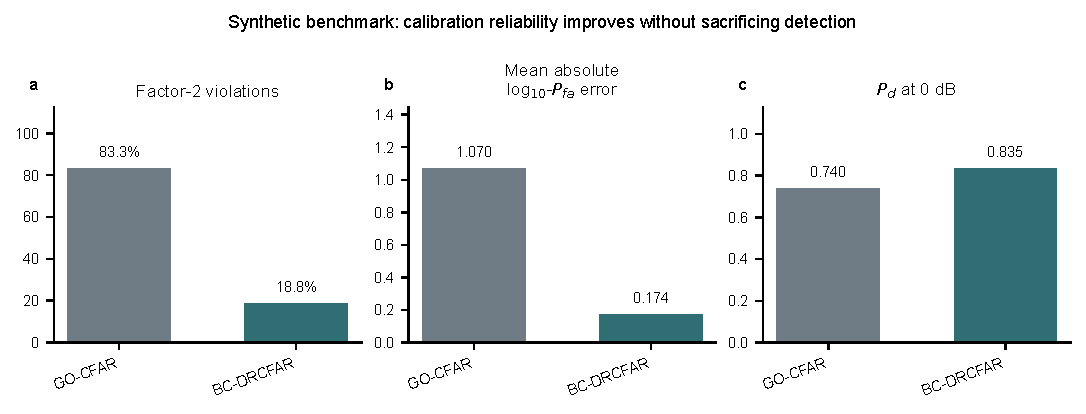
\includegraphics[width=\textwidth]{fig2_synthetic_calibration.pdf}
\caption{Synthetic calibration result at the nominal operating point.
BC-DRCFAR reduces acquisition-level false-alarm excursions and log-scale
calibration error while preserving target detection at 0 dB.}
\label{fig:synthetic-calibration}
\end{figure}
\FloatBarrier

The main improvement is acquisition-level calibration reliability.
The pooled $P_{\mathrm{fa}}$ confirms that the declared operating point is
matched on average, while the factor-2 metric shows how often individual
conditions remain close to that point. The drop from 83.3\% to 18.8\% means that
BC-DRCFAR suppresses the acquisition-specific false-alarm bursts that are
hidden by pooled summaries. The simultaneous increase in $P_{\mathrm{d}}$ at
0 dB shows that the calibration gain is obtained while retaining weak-target
detection performance.

The synthetic result is the strongest evidence for the calibration mechanism
because the sources of nonstationarity are controlled. Each clutter family
changes a different part of the background: tail weight, correlation, mixture
composition, contamination, or state transition. A scalar threshold factor has
to absorb these changes through one number. BC-DRCFAR instead receives a
descriptor vector from the same reference background and can adjust the
threshold according to the mechanism expressed in that vector. The improvement
in both log-$P_{\mathrm{fa}}$ error and factor-2 violations is therefore
consistent with the intended role of the background branch. The main numerical
comparison is reported in Table~\ref{tab:synthetic}.

\begin{table}[!htbp]
\centering
\small
\caption{Primary synthetic benchmark summary at the nominal operating point.}
\label{tab:synthetic}
\begin{tabularx}{\textwidth}{lYYYY}
\toprule
Method & Pooled $P_{\mathrm{fa}}$ & Factor-2 violation & MAE log10-$P_{\mathrm{fa}}$ & $P_{\mathrm{d}}$ at 0 dB \\
\midrule
GO-CFAR & -- & 0.833 & 1.070 & 0.740 \\
BC-DRCFAR & 0.01012 & 0.188 & 0.174 & 0.835 \\
\bottomrule
\end{tabularx}
\end{table}
\FloatBarrier

\subsection{Retrospective IPIX: feature-head calibration improves reliability}
\label{subsec:ipix-results}

The retrospective IPIX cohort showed the same calibration pattern. With frozen
calibration artifacts, the feature head produced a macro $P_{\mathrm{fa}}$ of
0.009998. Its acquisition-level absolute
log-$P_{\mathrm{fa}}$ error was 0.199, compared with 0.213 for scalar
calibration and 0.299 for GO-CFAR. The feature head satisfied the acquisition
factor-2 condition in 7 of 9 acquisitions. The primary detection probability was
0.282, close to the GO-CFAR value of 0.286. The measured-data gain lay mainly in
false-alarm calibration, with little change in the detection trade-off.

Figure~\ref{fig:ipix-acquisition} places the retrospective IPIX result at the
acquisition level. The panels separate acquisition-level false-alarm error,
factor-2 status, and primary-bin $P_{\mathrm{d}}$, making the real-data
calibration gain visible across the nine acquisition-disjoint files.

\begin{figure}[!htbp]
\centering
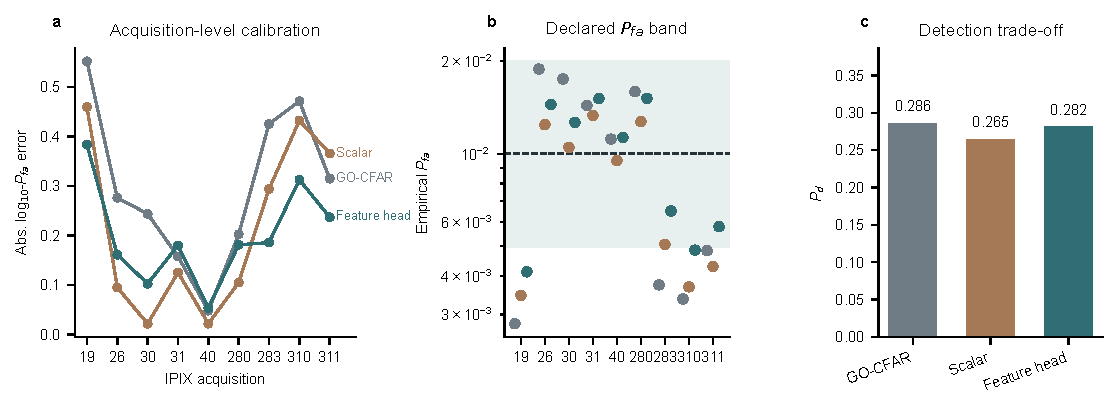
\includegraphics[width=\textwidth]{fig3_ipix_acquisition.pdf}
\caption{Retrospective IPIX acquisition-level result. Frozen calibration
artifacts are applied to nine acquisition-disjoint measured sea-clutter files,
with performance summarized by acquisition-level false-alarm calibration and
primary-bin detection probability.}
\label{fig:ipix-acquisition}
\end{figure}
\FloatBarrier

The retrospective result is important because all evaluated acquisitions are
scored with frozen feature-head and scalar calibration artifacts. Under that
protocol, scalar calibration improved over GO-CFAR, and the feature head gave
the lowest acquisition-level log error. This ordering matches the design of
BC-DRCFAR. A scalar correction shifts the threshold globally; the feature head
responds to the background descriptors of each acquisition. The result is a
measured-data trade-off with stronger false-alarm calibration and
$P_{\mathrm{d}}$ close to GO-CFAR.

The IPIX result adds the measured-data test beyond the controlled synthetic
benchmark. The acquisitions differ in their empirical clutter statistics, target
range bins, and polarization behaviour, but they are evaluated with the same
declared operating point and frozen calibration artifacts. The feature head
keeps the macro false-alarm probability nearly nominal and improves the
acquisition-level log error over GO-CFAR. The small change in primary
$P_{\mathrm{d}}$ is also informative: the reliability gain is achieved mainly
through false-alarm calibration while the target-separation behaviour remains
close to the GO-CFAR reference. Table~\ref{tab:ipix} gives the measured-data
calibration trade-off across the development and retrospective settings.

\begin{table}[!htbp]
\centering
\small
\caption{Retrospective IPIX calibration trade-off. The feature head is the main
external-acquisition reliability result, while scalar and low-rank variants are
mechanistic comparisons.}
\label{tab:ipix}
\begin{tabularx}{\textwidth}{lYYYY}
\toprule
Family & Macro $P_{\mathrm{fa}}$ & Factor-2 metric & Primary $P_{\mathrm{d}}$ & Abs. log10 error \\
\midrule
Development scalar & 0.009792 & 0.845 & 0.375 & 0.278 \\
Development low-rank & 0.011479 & 0.200 & 0.393 & -- \\
Retrospective scalar & 0.008332 & 0.830 & 0.265 & 0.213 \\
Retrospective feature head & 0.009998 & 0.846 & 0.282 & 0.199 \\
\bottomrule
\end{tabularx}
\end{table}
\FloatBarrier

\subsection{Ablations: background descriptors drive the calibration gain}
\label{subsec:ablation-results}

Feature ablation shows that the full background-conditioned head is the most
stable deployable choice. Removing anchor features or polarization information
degrades the external trade-off, whereas removing uncertainty or series-shift
features has a smaller effect. Anchor features provide the strongest reference
for the operating-point scale, and polarization information adds acquisition
context beyond a global scalar correction. The ablation pattern ties the gain to
structured background descriptors instead of generic model capacity.

The ablation results also clarify how the background is used. Anchor features
provide a stable reference for the nominal false-alarm scale. Polarization
features carry acquisition context that changes the distribution of clutter
returns and the way high-amplitude reference cells should be interpreted.
Uncertainty and series-shift descriptors refine this context, but their removal
has a smaller effect in the evaluated setting. The full feature head therefore
combines a stable operating-point anchor with acquisition-specific background
information.

This ablation pattern supports the central design choice. The full head is not
explained by a single decorative feature group. Anchor and polarization features
carry the strongest external-acquisition signal, while the auxiliary descriptors
preserve a compact description of uncertainty and series displacement. The
background-conditioned family remains close across several ablations, showing
that the gain is distributed across calibration features and remains stable
across multiple descriptor choices.

\subsection{Temporal and external audits: reliability remains traceable}
\label{subsec:boundary-results}

The long-horizon holdout shows how calibration behaves under temporal drift.
Scalar calibration changed from early $P_{\mathrm{d}}=0.4663$ to late
$P_{\mathrm{d}}=0.2625$, while the feature head changed from 0.4742 to 0.2782.
Under the same split, the feature head reduced the worsening in calibration
error. Fold-level audits identified real source difficulty in the hardest folds,
beyond sample-count imbalance. Domain audits placed IPIX inside the learned
acceptance region, and the external-domain checks provided a reproducible
transfer evaluation beyond the main IPIX setting.

These audits make the reliability result traceable. The long-horizon split
shows that temporal drift affects both detection and calibration in measured
sea clutter. The feature head reduces the calibration worsening under the same
temporal split, matching the behaviour targeted by background conditioning. The
fold-level audit links difficult folds to source structure, and the
external-domain checks document how far the current calibration evidence can be
followed beyond the main IPIX evaluation. Table~\ref{tab:boundary} summarizes
the ablation and reliability checks that support this mechanism.

Figure~\ref{fig:mechanism-audit} provides the mechanism-level counterpart to
Table~\ref{tab:boundary}. It links feature ablation, long-horizon drift,
source-fold structure, and external-domain transfer into one reliability chain,
showing that the calibration gain is tied to background information rather than
to a single split or a single reporting metric.

\begin{figure}[!htbp]
\centering
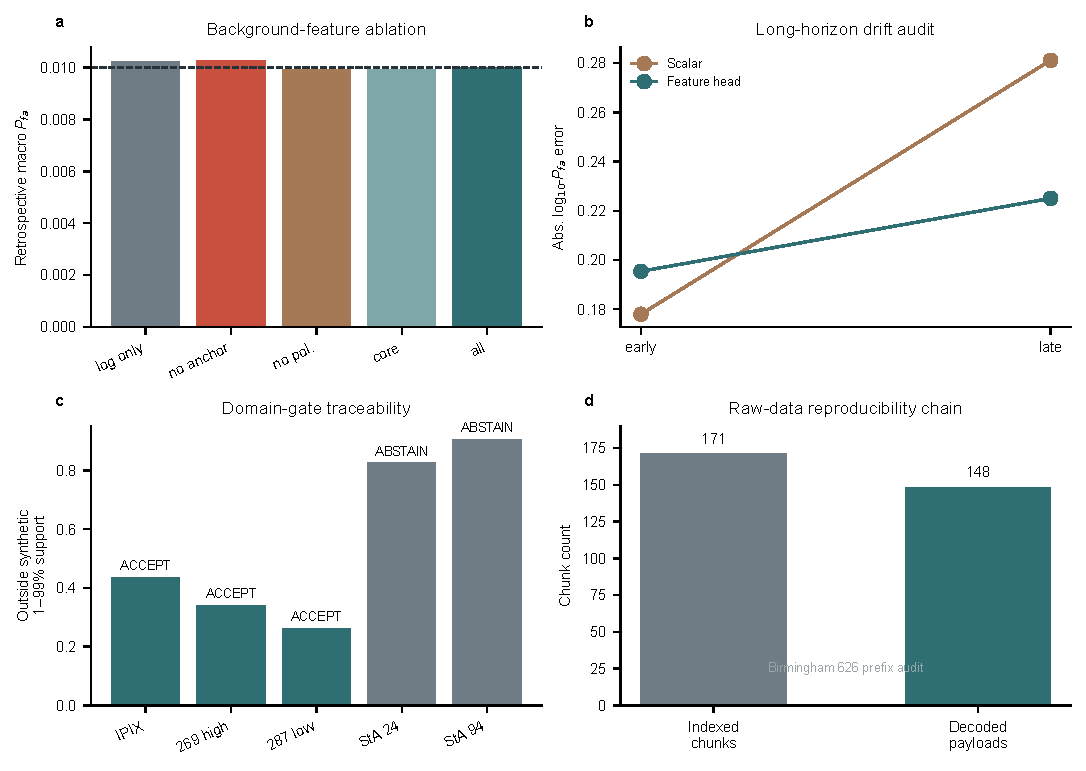
\includegraphics[width=\textwidth]{fig4_mechanism_audit.pdf}
\caption{Mechanism and reliability audit. Background-feature ablations are
presented together with temporal, source, and external-domain checks to show how
acquisition-conditioned calibration produces the observed false-alarm
reliability gain.}
\label{fig:mechanism-audit}
\end{figure}
\FloatBarrier

\begin{table}[!htbp]
\centering
\small
\caption{Ablation and reliability audit summary. The table combines mechanism
checks from feature ablation with temporal, source, and external-domain
reliability audits.}
\label{tab:boundary}
\begin{tabularx}{\textwidth}{lXX}
\toprule
Check & Result & Interpretation \\
\midrule
Feature ablation & Removing anchor features or polarization information changes
the external trade-off more than removing auxiliary uncertainty or series-shift
terms & Anchor and polarization descriptors carry the strongest calibration
context \\
Background-conditioned family & Several ablated feature-head variants remain
close to the full model on retrospective macro $P_{\mathrm{fa}}$ and
$P_{\mathrm{d}}$ & The calibration gain is distributed across background
features and remains stable across descriptor choices \\
Long-horizon IPIX holdout & Feature head softens calibration drift under
temporal split & Temporal reliability audit \\
Fold 3/4 source audit & Difficult folds reflect genuine source difficulty &
Source-difficulty audit \\
Birmingham 626 & 148 prefix chunks decoded from 171 indexed records & Raw-data
reproducibility audit \\
St Andrews/domain audits & External-domain checks evaluate transfer reliability
& Domain-reliability audit \\
\bottomrule
\end{tabularx}
\end{table}
\FloatBarrier

\section{Discussion}
\label{sec:discussion}

BC-DRCFAR advances CFAR detection by treating false-alarm calibration as a
background-conditioned decision problem. In nonstationary sea clutter, the
reference background is more than a local power estimate. Its distribution,
temporal dependence, tail behaviour, and ordered reference structure all affect
whether a declared $P_{\mathrm{fa}}$ remains reliable within an acquisition.

This framing changes the role of the reference window. In classical CFAR, the
reference cells mainly supply the local clutter level used to scale a threshold.
In BC-DRCFAR, the same cells also describe the calibration condition. A
heavy-tailed background, a shifted reference series, or a temporally persistent
clutter state is treated as information about how the threshold should be set.
That is the central methodological contribution: CFAR calibration is made
conditional on the background actually seen by the detector.

This view separates BC-DRCFAR from the usual extensions of classical CFAR.
CA-CFAR, GO-CFAR, SO-CFAR, and OS-CFAR retain a clear thresholding
interpretation, but their reference-window summaries are exposed to heavy-tailed,
heterogeneous, and mismatched clutter
\cite{hansen1980go,rohling1983cfar,barkat1989multiple}. Adaptive and statistical
CFAR methods address this problem through richer clutter models, robust
reference processing, and multi-feature probability models
\cite{xue2022adaptive,zhao2019dbscan,wen2024gev,li2025copula,jiang2025twodcfar}.
BC-DRCFAR keeps the declared false-alarm probability as the operating language
and makes the threshold calibration depend on the observed background. The
contribution is a calibrated extension of CFAR to acquisition-specific
sea-clutter structure.

The comparison also explains why acquisition-level false-alarm summaries are
central to this problem. Pooled $P_{\mathrm{fa}}$ gives the average operating
point, while individual acquisitions reveal how consistently the detector holds
that point under changing clutter. The factor-2 violation rate and log-scale
false-alarm error used here make that behaviour visible. BC-DRCFAR is designed
around those acquisition-level quantities, which is why its main advantage
appears in reliability metrics as well as in the pooled rate.

The comparison with feature-based and learning-based detectors is equally
important. Multi-domain feature fusion, reconstruction models, and manifold or
geometric detectors mainly improve target--clutter separability in complex
maritime scenes \cite{wen2022spatiotemporal,wang2025twostage,chen2026mspmig}.
BC-DRCFAR instead puts the operating point at the centre of the model. Its score
branch orders target evidence, while the feature head uses background
descriptors to set the threshold for the declared $P_{\mathrm{fa}}$. This
division explains the retrospective IPIX result: the main gain appears in
acquisition-level false-alarm calibration, with the primary detection
probability remaining close to GO-CFAR.

This division of labour is useful for radar deployment. Operators choose a
false-alarm operating point because it has operational meaning. BC-DRCFAR keeps
the score and calibration tasks connected but distinct. The score branch
captures target evidence; the feature head translates the declared operating
point into the threshold required by the observed clutter.

Against the comparison set of recent sea-clutter detectors, the main innovation
is therefore the placement of learned background representation inside the CFAR
calibration step. Feature-fusion and reconstruction detectors improve the
evidence score; copula and statistical CFAR methods improve the probability
model; classical CFAR variants improve reference-window robustness. BC-DRCFAR
adds an acquisition-conditioned map from declared $P_{\mathrm{fa}}$ to the
decision threshold. That map is what lets the method preserve the CFAR operating
language while responding to measured background structure
\cite{wen2022spatiotemporal,liang2022unsupervised,li2025copula,jiang2025twodcfar,chen2025multidomain}.

Figure~\ref{fig:method-position} makes this positioning explicit. The comparison
matrix separates the operating interface, background representation, evidence
modelling, threshold calibration, and acquisition-level reliability roles:
classical and statistical CFAR methods strengthen the reference-window or
probability model, feature and reconstruction detectors strengthen the evidence
score, and BC-DRCFAR inserts learned background representation into the
threshold-calibration step that controls the declared operating point.

\begin{figure}[!htbp]
\centering
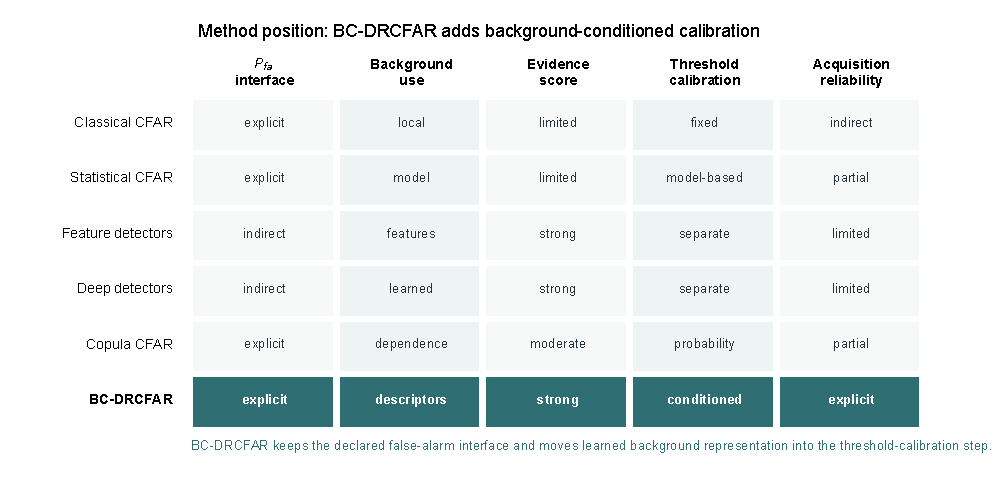
\includegraphics[width=\textwidth]{fig5_method_position.pdf}
\caption{Position of BC-DRCFAR relative to recent sea-clutter detection methods.
The comparison matrix highlights the central contribution of the method: learned
background representation is inserted into the CFAR threshold-calibration step
while the declared false-alarm operating point remains the decision interface.}
\label{fig:method-position}
\end{figure}
\FloatBarrier

The experiments support this mechanism across controlled and measured settings.
On the synthetic benchmark, BC-DRCFAR reduces factor-2 false-alarm violations and
log-$P_{\mathrm{fa}}$ error while improving $P_{\mathrm{d}}$ at 0 dB. On
retrospective IPIX acquisitions, frozen feature-head calibration keeps macro
$P_{\mathrm{fa}}$ near the nominal value and improves acquisition-level error
over scalar calibration and GO-CFAR. The ablations point to the same conclusion:
anchor features and polarization information carry calibration context that a
background-conditioned threshold head can use directly.

The reliability audits add the deployment perspective. The long-horizon split
shows that temporal drift changes both detection probability and calibration
error, while background conditioning softens the calibration drift. Fold-level
audits show that the hardest folds reflect genuine source difficulty and
sample-count structure. Birmingham 626 adds a raw-data reproducibility check: the
remote ZIP, MAT/HDF5 schema, B-tree chunk index, and chunk payloads can be traced
to decoded complex IQ blocks. That traceable path extends the evidence chain for
acquisition-level CFAR calibration.

Taken together, the experiments support a clear contribution to radar signal
processing: background-conditioned calibration turns CFAR from a local
thresholding recipe into an acquisition-aware reliability mechanism. The method
retains the declared false-alarm interface that makes CFAR practical, and adds a
data-driven threshold calibration rule tied to the clutter state. This is the
step that connects modern feature representation with the operational discipline
of false-alarm control.

This framing also clarifies the role of the reliability audits. The audits are
part of the same evidence chain. The synthetic benchmark verifies the mechanism
under controlled clutter shifts. The retrospective IPIX study tests frozen
calibration on measured sea clutter. The ablations identify which background
information drives the calibration behaviour. The temporal and source audits
show how the same decision rule behaves when acquisition conditions change.
Together these experiments support BC-DRCFAR as a calibrated radar
signal-processing method whose reliability evidence is tied to its calibration
mechanism.

\section{Conclusion}
\label{sec:conclusion}

BC-DRCFAR addresses acquisition-level false-alarm instability by conditioning
CFAR calibration on the observed clutter background. It keeps the declared
$P_{\mathrm{fa}}$ as the operating point, then uses background descriptors and a
feature-head threshold to adapt the decision rule to nonstationary sea clutter.
The scale-equivariant score branch preserves target-evidence ordering while the
calibration branch sets the acquisition-specific threshold.

Controlled and measured evaluations give the same conclusion. On the synthetic
benchmark, BC-DRCFAR reduces the factor-2 violation rate from 83.3\% to 18.8\%,
lowers the mean absolute log10-$P_{\mathrm{fa}}$ error from 1.070 to 0.174, and
raises $P_{\mathrm{d}}$ at 0 dB from 0.740 to 0.835. On retrospective IPIX
acquisitions, the feature head keeps the macro false-alarm probability near the
nominal level and satisfies the acquisition factor-2 condition in 7 of 9
acquisitions. The ablation and reliability audits point to the same mechanism:
background-conditioned calibration gives CFAR a practical route to reliable
radar target detection in nonstationary sea clutter.

\section*{CRediT authorship contribution statement}

Zixuan Liu: conceptualization, methodology, software, formal analysis,
investigation, visualization, writing - original draft. Wei Xiong:
conceptualization, validation, supervision, writing - review and editing,
project administration.

\section*{Declaration of competing interest}

The authors declare that they have no known competing financial interests or
personal relationships that could have appeared to influence the work reported
in this paper.

\section*{Data and code availability}

The manuscript uses public radar data sources and project-generated synthetic
benchmarks. The IPIX radar data are available from the McMaster University IPIX
archive, and the Birmingham 626 raw-data audit uses publicly released maritime
radar data. The processed evaluation summaries, synthetic benchmark
configuration, and analysis code supporting the reported figures and tables are
available from the corresponding author upon reasonable request.

\section*{Acknowledgements}

This work was supported in part by the National Natural Science Foundation of
China (62202148). It was also supported by the Natural Science Foundation of
Hubei Province (2022CFB908 and 2019CFB530). It was also supported by the China
Scholarship Council (201808420418). The authors gratefully acknowledge these
funding sources. The funders had no role in study design, data collection and
analysis, decision to publish, or preparation of the manuscript. The authors
thank the open benchmark and radar data communities whose public materials
supported the study.

\bibliographystyle{elsarticle-num}
\bibliography{refs}

\end{document}
